\begin{frame}[t]{}
		\begin{minipage}[]{0.7\columnwidth}
	\centering
		\Huge MD シミュレーションによる\\ネットワークポリマーの緩和挙動  \\[10mm]
		\Large 東亞合成 $\bigcirc$佐々木裕 \\
	\end{minipage}
	\begin{minipage}[]{0.29\columnwidth}
		\begin{figure}\centering
			
\includegraphics[width=\columnwidth]{toa_logo.png}
		\end{figure}
	\end{minipage}
		\vspace{10mm}
		% \large
\begin{itembox}[l]{ABSTRACT}
	Existence of mechanical hysteresis is believed to be one of a key to achieve high durability for rubber materials.
	For hysteresis cycle, added fillers are believed to play an important roll in meso-scale region response against local stress.
	Our question is ``Is there any other mechanism to enhance durability in micro-scale region such as size of polymer chains?''.

	``Phantom Network Model'', in which fluctuation of junction point is rather high, seems to be a good candidate for micro-scale energy dissipation.
	Introducing random connectivity for network junctions, previously we successfully presented ``Phantom Network Model'' in molecular dynamics simulations.

	In this presentation, relationship of mechanical hysteresis and relaxation characteristics of ``Phantom Network Model'' was investigated.
\end{itembox}

		\begin{block}{はじめに}
			\begin{columns}[T]
				\begin{column}{.33\linewidth}
					\begin{itemize}
						\item 高分子材料の破壊耐性向上の設計指針
						\item 耐久性、可逆性に優れたゴム材料
						\item 破壊工学的$\Rightarrow$クラック進展を抑制
					\end{itemize}
					\centering
					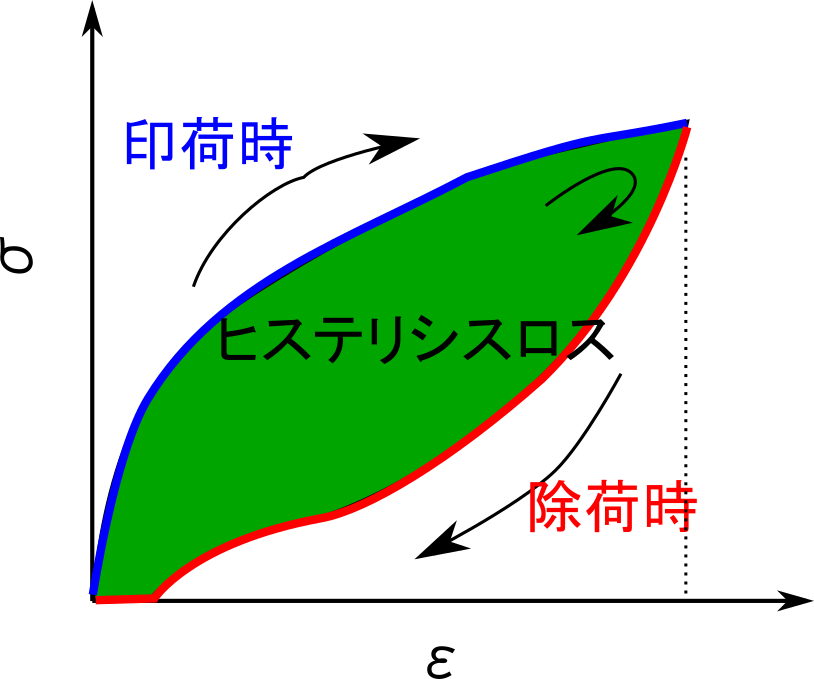
\includegraphics[width=.4\textwidth]{hysteresis_curve.png} 
				\end{column}
				\begin{column}{.33\linewidth}
					\begin{itembox}[l]{Andrews 理論\cite{andrews}}
						\begin{columns}[totalwidth=.9\textwidth]
							\column{.75\textwidth}
								クラックの微小進展時に、
								\begin{itemize}
								\item
								\textcolor{blue}{Loading 場とUnloading 場}
								\item
								\alert{この差}が、全体の変形に要したエネルギーを\alert{散逸}
								\item
								鎖破断のエネルギーが低減 \\$\Rightarrow$ \alert{強靭さの起源。}
								\end{itemize}	
							\column{.24\textwidth}
								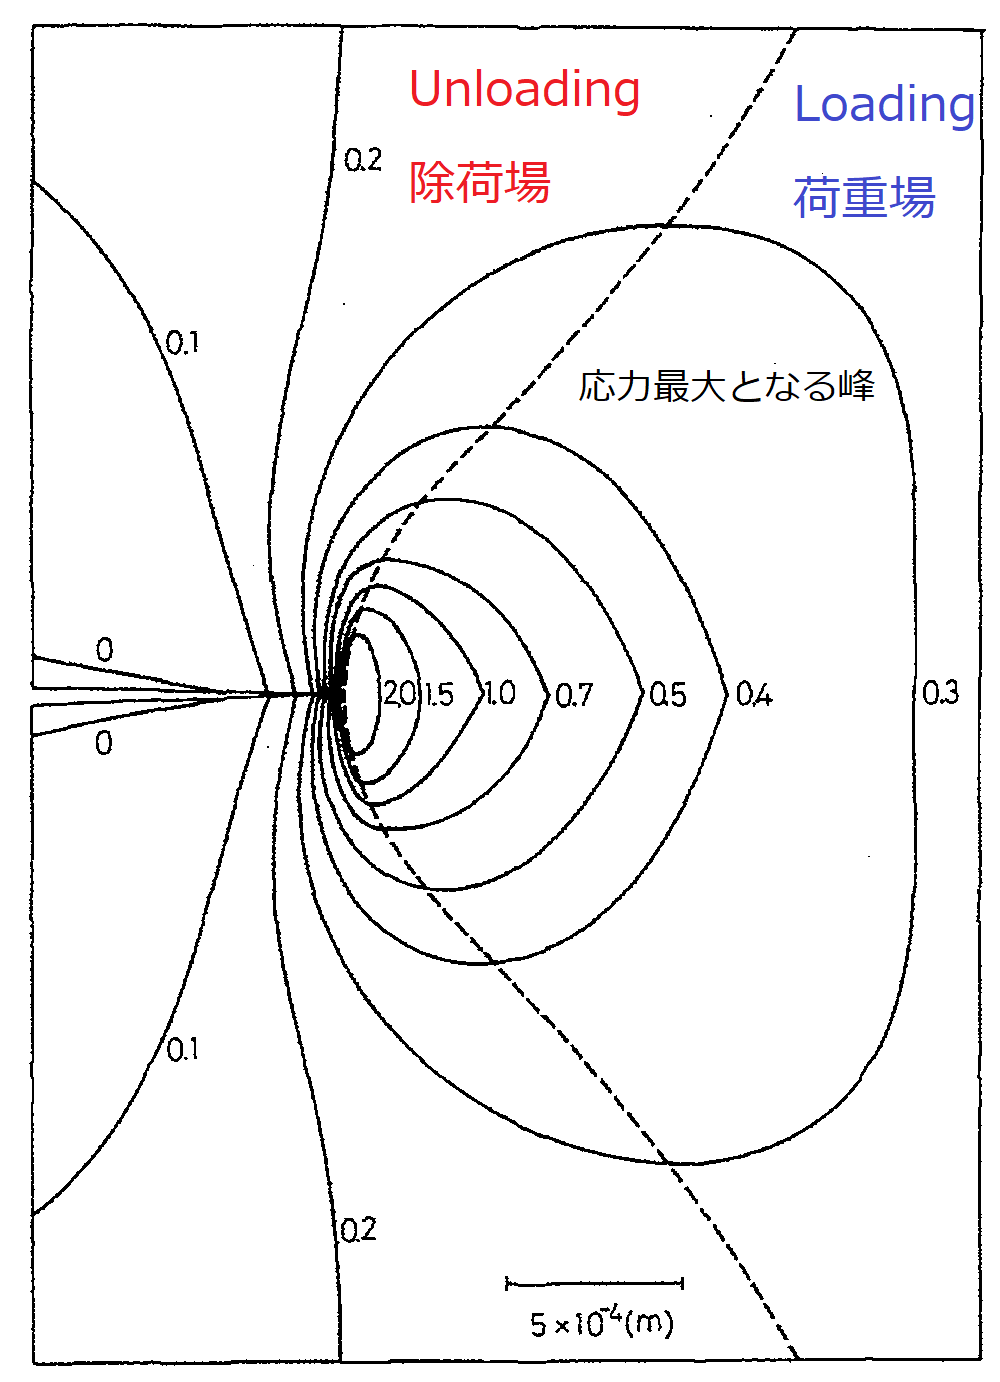
\includegraphics[width=.9\textwidth]{crack.png}     
						\end{columns}
					\end{itembox}
				\end{column}
				\begin{column}{.33\linewidth}
					\begin{itembox}[l]{ランダム構造とは?}
						\begin{columns}[totalwidth=.9\textwidth]
							\column{.6\textwidth}
									\begin{itemize}
										\item 連結性を不均一に
											\begin{itemize}
												\item 連結に\alert{位置依存性}
											\end{itemize}
										\item 巨視的な変形後
											\begin{itemize}
												\item 結節点のゆらぎが不均一
												\item 多様な緩和モード
												% \item \alert{緩和の長時間化?}
											% \item ファントムネットワークモデルの諸特性の発現?
											\end{itemize}
										% \item \alert{解析を容易}に、
										% 	\begin{itemize}
										% 		\item 既往研究で反応系
										% 		\item ストランド長と結合数を一定
										% 	\end{itemize}
									\end{itemize}
							\column{.35\textwidth}
								% ランダム構造の模式図
								% \vspace{10mm}
								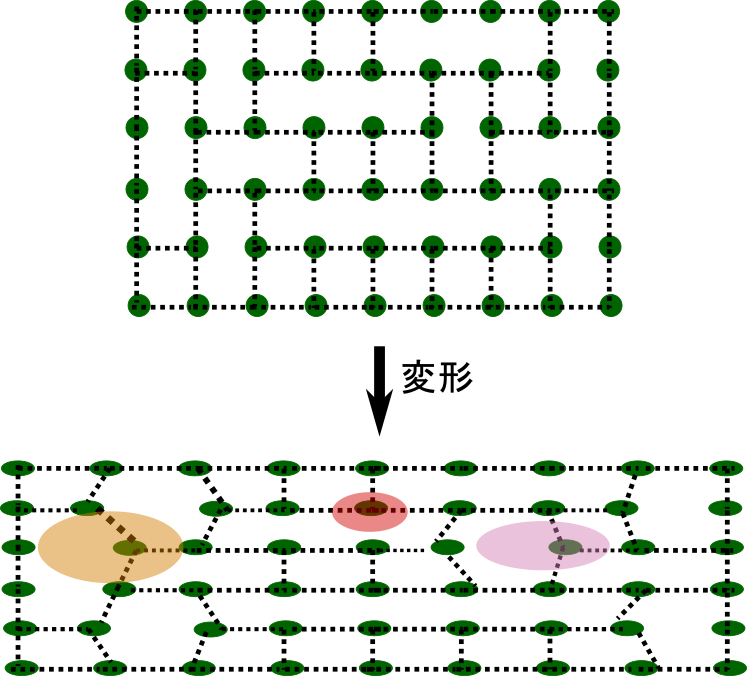
\includegraphics[width=\textwidth]{random_NW.png}
						\end{columns}
					\end{itembox}
				\end{column}
			\end{columns}
		\end{block}
		

		\begin{columns}[T]
			\begin{column}{.49\linewidth}
				\begin{block}{はじめに}
					% \begin{columns}[totalwidth=.9\linewidth]
%     \column{\textwidth}
%         \begin{itembox}[c]{高分子材料でマルチマテリアル化}
%             \begin{itemize}
%                 \item 高い比強度の有効利用
%                 \item {\color{red} 「接着接合」}への高分子の利用
%                     \begin{itemize}
%                         \item 柔らかさを生かした{\color{red} 「弾性接着接合」}
%                         \item 耐久性、可逆性に優れた\alert{ゴム材料に注目}
%                     \end{itemize}
%                 \item {\color{blue}耐久性が不明確(特に疲労破壊に対して)}
%             \end{itemize}
%         \end{itembox}
% \end{columns}

\begin{columns}[totalwidth=.9\linewidth]
    \column{\textwidth}
        \begin{boxnote}
            \textbf{高分子材料でマルチマテリアル化 $\Leftrightarrow$ 高い比強度の有効利用}
            \begin{itemize}
                \item {\color{red} 「接着接合」}への高分子の利用
                    \begin{itemize}
                        \item 柔らかさを生かした{\color{red} 「弾性接着接合」}
                        \item 耐久性、可逆性に優れた\alert{ゴム材料に注目}
                    \end{itemize}
                \item {\color{blue}耐久性が不明確}
                    \begin{itemize}
                        \item 特に疲労破壊に対して
                    \end{itemize}
            \end{itemize}
        \end{boxnote}
\end{columns}

\begin{columns}[totalwidth=.9\linewidth]
    \column{\textwidth}
    \begin{itembox}[l]{ヒステリシスと破壊靭性}
        \begin{columns}[totalwidth=\linewidth]
            \column{.8\textwidth}
                \begin{itemize}
                    \item 力学的ヒステリシス
                    \begin{itemize}
                        \item
                        印荷時に比べて、除荷時の応力が低下する減少
                        \item
                        ヒステリシスロス:変形時のエネルギー散逸
                    \end{itemize}
                    \item 破壊靭性との関係
                    \begin{itemize}
                        \item
                        Andrews 理論:ヒステリシスロスの重要性が指摘
                    \end{itemize}
                \end{itemize}
            \column{.2\textwidth}
                \centering
                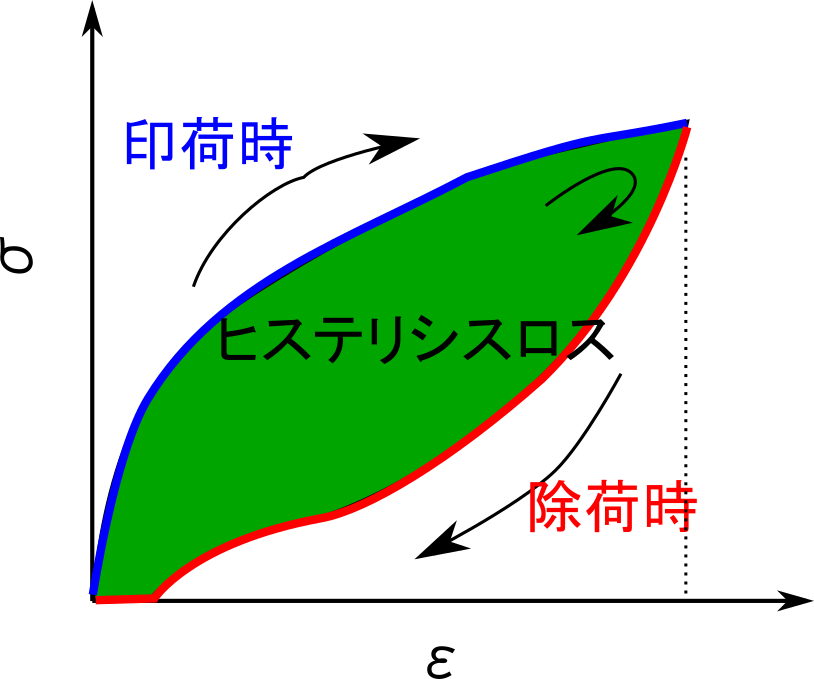
\includegraphics[width=\textwidth]{hysteresis_curve.png}
            \end{columns}
    \end{itembox}
\end{columns}

\begin{columns}[totalwidth=.9\linewidth]
    \column{\textwidth}
    \begin{itembox}[l]{Andrews 理論\cite{andrews}}
        \begin{columns}[totalwidth=\textwidth]
            \column{.8\textwidth}
                クラックの微小進展時に、
                \begin{itemize}
                    \item
                    \textcolor{red}{Loading 場}と\textcolor{blue}{Unloading 場}のひずみエネルギーの差
                    \item
                    全体の変形に要したエネルギーの多くを\textcolor{red}{散逸}
                    \item
                    鎖の破断へのエネルギーが低減 $\Rightarrow$ \alert{強靭さの起源。}
                \end{itemize}	
            \column{.2\textwidth}
                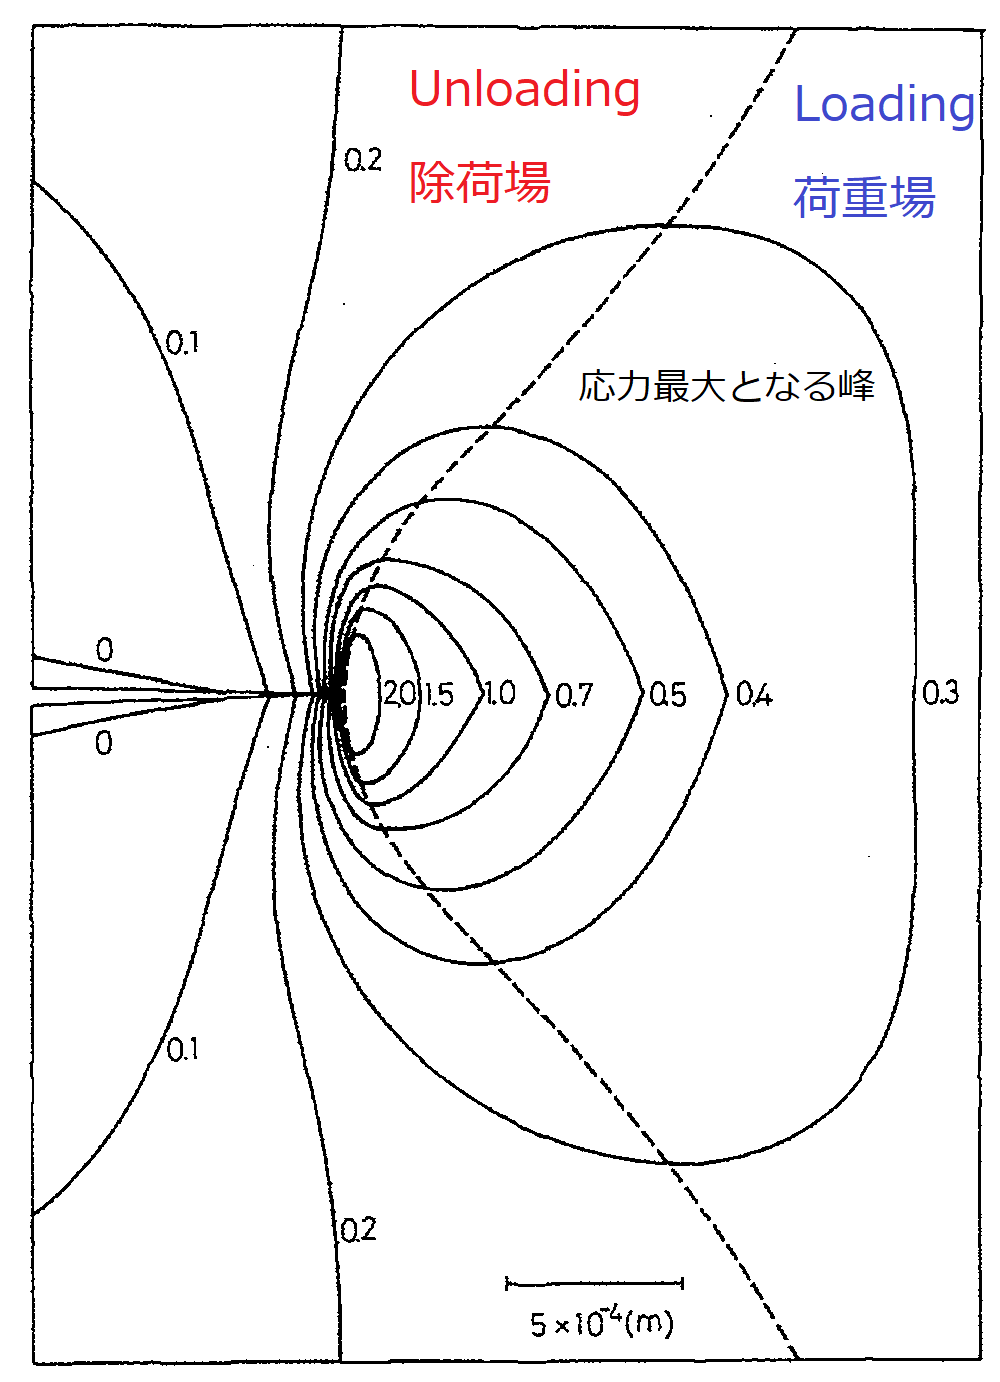
\includegraphics[width=.8\textwidth]{crack.png}     
        \end{columns}
    \end{itembox}
\end{columns}

\begin{columns}[totalwidth=.9\linewidth]
    \column{\textwidth}
    \begin{itembox}[l]{架橋点の環境とランダムな接続性}
        \begin{columns}[totalwidth=\textwidth]
			\column{.3\textwidth}
                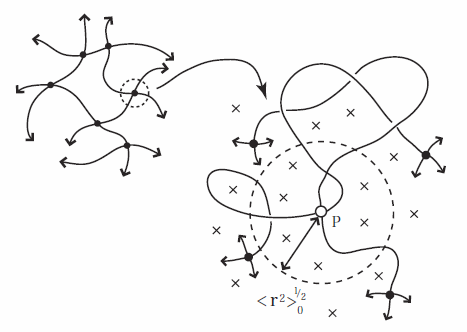
\includegraphics[width=\textwidth]{JP_vicinity.png}
                架橋点は、\alert{多数のストランド(図中の×)}に囲まれている。
			\column{.4\textwidth}
                \begin{itemize}
                    \item 接続性を不均一に
                        % \begin{itemize}
                        %     \item 接続に\alert{位置依存性}
                        % \end{itemize}
                    \item 巨視的な変形後
                        \begin{itemize}
                            \item \alert{結節点のゆらぎが不均一}
                            \item 多様な緩和モード
                            % \item \alert{緩和の長時間化?}
                        \item ファントムネットワークの\\諸特性が発現
                        \end{itemize}
                \end{itemize}
            \column{.3\textwidth}
				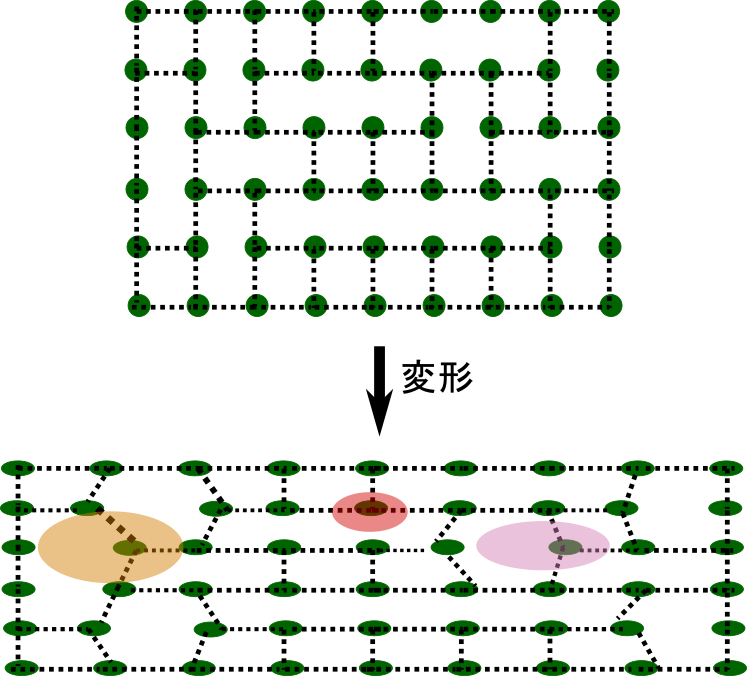
\includegraphics[width=.8\textwidth]{random_NW.png}
		\end{columns}
    \end{itembox}
\end{columns}
				\end{block}
				\begin{block}{ランダム構造について}
					\centering
\begin{columns}[totalwidth=.9\textwidth]
    \column{.6\textwidth}
            \begin{itemize}
                \item 連結性を不均一に
                    \begin{itemize}
                        \item 連結に\alert{位置依存性}
                    \end{itemize}
                \item 巨視的な変形後
                    \begin{itemize}
                        \item 結節点のゆらぎが不均一
                        \item 多様な緩和モード
                        \item \alert{緩和の長時間化?}
                    % \item ファントムネットワークモデルの諸特性の発現?
                    \end{itemize}
                \item \alert{解析を容易}に、
                    \begin{itemize}
                        \item 既往研究で反応系
                        \item ストランド長と結合数を一定
                    \end{itemize}
            \end{itemize}
    \column{.35\textwidth}
        ランダム構造の模式図
        \vspace{10mm}
        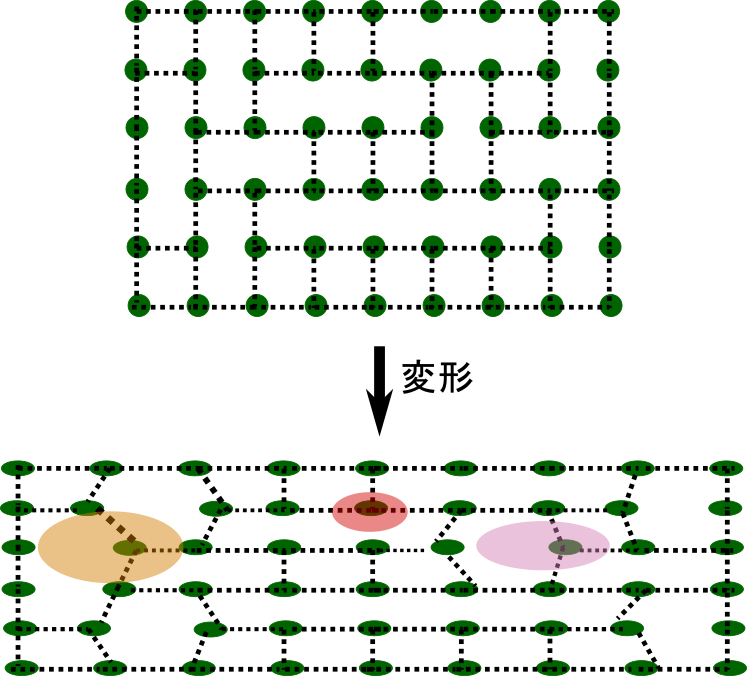
\includegraphics[width=\textwidth]{random_NW.png}
\end{columns}
				\end{block}
				\begin{block}{第三セクション}
					% \input{third}
				\end{block}
				\end{column}
				\begin{column}{.49\linewidth}
				\begin{block}{第四セクション}
					% \input{forth}
				\end{block}
				\begin{block}{参考文献}
					\begin{thebibliography}{99}
    \bibitem{andrews} E. H. Andrews, Y. Fukahori, J. of Mat. Sci., 12, 1307 (1977)
    \bibitem{smith} T. L. Smith, R. A. Dickie, J. of Polym. Sci. A-2: Polym. Phys., 7, 635 (1969)
    \bibitem{flory} P. J. Flory, Proc. R. Soc. London. Series A, 351, 351 (1976)
    \bibitem{sasaki} 佐々木裕, 第69回レオロジー討論会 (2021)
    \bibitem{Auhl} R. Auhl et al., J. of Chem. Phys., 119, 12718 (2003)
    \bibitem{Kroger} S. Shanbhag, M. Kr\"{o}ger, Macromol. 40 2897 (2007)
    \bibitem{rubinstein} J. T. Kalathi et al., Macromol. 47 6925 (2014)
\end{thebibliography}
				\end{block}
			\end{column}
		\end{columns}
		\end{frame}